\section{ILUC Recognition} \label{sec:iluc_recognition}
This section describes a novel algorithm that allows the LUA software to recognize the ILUC. The algorithm combines the lines and edges coming from the profile analysers to form a 3-dimensional representation of the ILUC, similar to how the pipes are already found. The goal of the algorithm is to find the ILUC's direction, radius and centre. For convenience, these values together are termed the \textit{ILUC face}.

The motivation to recognise the ILUC face lies in the ability to perform an accurate pre-line up of the new joint and main line. The new joint's position and orientation can be preemptively adjusted to the ILUC face during line up (see \ref{fig:oop_ILUC_ribs}). This ultimately leads to a more accurate and efficient line up of the new joint and main line, since the ILUC is always centered and fixed in the main line.

The ILUC consists of ten ribs (see \cref{fig:iluc,fig:oop_lua}), each of which is recognised by the profile analysers as a line segment of a specific length ($\sim 1$ cm). In turn, each of these line segments generates two edge points. Consequently, all five profile analysers together can generate up to
\begin{align*}
           & 5 \text{ profile analyser threads}         \\
    \times & 10 \text{ ILUC ribs per profile analyser}  \\
    \times & 2 \text{ ILUC rib edge point per ILUC rib} \\
    =      & 100 \text{ ILUC rib edge points}.
\end{align*}
These edge points are used in algorithm \ref{alg:iluc_recognition} to obtain an estimate of the ILUC face.
\begin{algorithm}
    \begin{algorithmic}[1]
        \State \textbf{function: } \lstinline[language=C]|multiSensorAnalyser_c::checkForILUCFace|
        \State Obtain ILUC rib edge points from the profile analysers
        \State \textbf{If} there are more than six edge points \textbf{then}
        \State \quad Run \lstinline[language=C]|multiSensorAnalyser_c::analyseILUCRibs| (see algorithm \ref{alg:iluc_estimation})
        \State \quad Store the ILUC face
        \State \quad \textbf{If} an ILUC face is found \textbf{then}
        \State \quad \quad Run \lstinline[language=C]|multiSensorAnalyser_c::fitILUCCylinder| (see algorithm \ref{alg:iluc_optimisation})
        \State \quad \quad \textbf{If} the optimised ILUC face has a lower error \textbf{then}
        \State \quad \quad \quad Overwrite the estimated ILUC face with the optimised ILUC face
        \State \quad \quad \textbf{end if}
        \State \quad \textbf{end if}
        \State \textbf{end if}
        \State \textbf{output: } ILUC face
    \end{algorithmic}
    \caption{Pseudo code for ILUC recognition.}
    \label{alg:iluc_recognition}
\end{algorithm}


\subsection{ILUC direction estimation}
The problem of estimating the ILUC face can be solved by combininh circle fits on the ILUC rib edges. The midpoints of these ILUC rib edge circle fits can be used to estimate the ILUC direction. The algorithm is described in algorithm \ref{alg:iluc_estimation}.
\begin{algorithm}[H]
    \begin{algorithmic}[1]
        \State \textbf{function} \lstinline[language=C]|multiSensorAnalyser_c::analyseILUCRibs|
        \State \textbf{input} ILUC rib edge points per profile analyser
        \State Naively group ILUC rib edge points into ILUC rib edges
        \State Fit circles to the ILUC rib edges, yielding ILUC rib midpoints
        \State Remove outliers from the set of ILUC rib midpoints
        \State Get an approximate ILUC direction by fitting a line through ILUC rib edge midpoints
        \State \textbf{If} an approximate ILUC direction is found \textbf{then}
        \State \quad Use approximate ILUC direction to correctly match ILUC rib edge points into edges
        \State \quad Fit circles to the ILUC rib edges, yielding ILUC rib midpoints
        \State \quad Remove outliers from the set of ILUC rib midpoints
        \State \quad Get a corrected ILUC direction by fitting a line through ILUC rib edge midpoints
        \State \quad Use corrected ILUC direction to perform a final circle fit, yielding the ILUC centre and radius and completing the ILUC face estimation
        \State \quad Calculate average error of the ILUC face
        \State \textbf{end if}
        \State \textbf{output: } ILUC face, ILUC rib edge points without outliers, average error
    \end{algorithmic}
    \caption{Pseudo code for ILUC face estimation.}
    \label{alg:iluc_estimation}
\end{algorithm}
In line 3 of algorithm \ref{alg:iluc_estimation} the ILUC rib edge points are grouped into ILUC rib edges based on their index in each of the profile analyser threads. This approach is naive, because it does not consider the possibility of a missing edge point. Missing edge points can occur due to a profile analyser not detecting an ILUC rib edge. There are multiple reasons a profile analyser might miss an edge, which are left out of the scope of this discussion.

Mismatched ILUC rib edges result in slanted circles. The midpoints resulting from the possibly mismatched set of ILUC rib edge points are used to obtain a first estimate of the ILUC direction. This estimate is then used to correctly match the ILUC rib edge points into edges. This allows for the correction of the ILUC direction. Finally, a circle fit is performed on all ILUC rib edge points (without outliers). This yields the ILUC centre and radius, completing estimation of the ILUC face.

A visual representation of the steps of algorithm \ref{alg:iluc_estimation} is shown in figure \ref{fig:iluc_estimation}.
\begin{figure}[H]
    \centering
    \begin{subfigure}[c]{0.45\textwidth}
        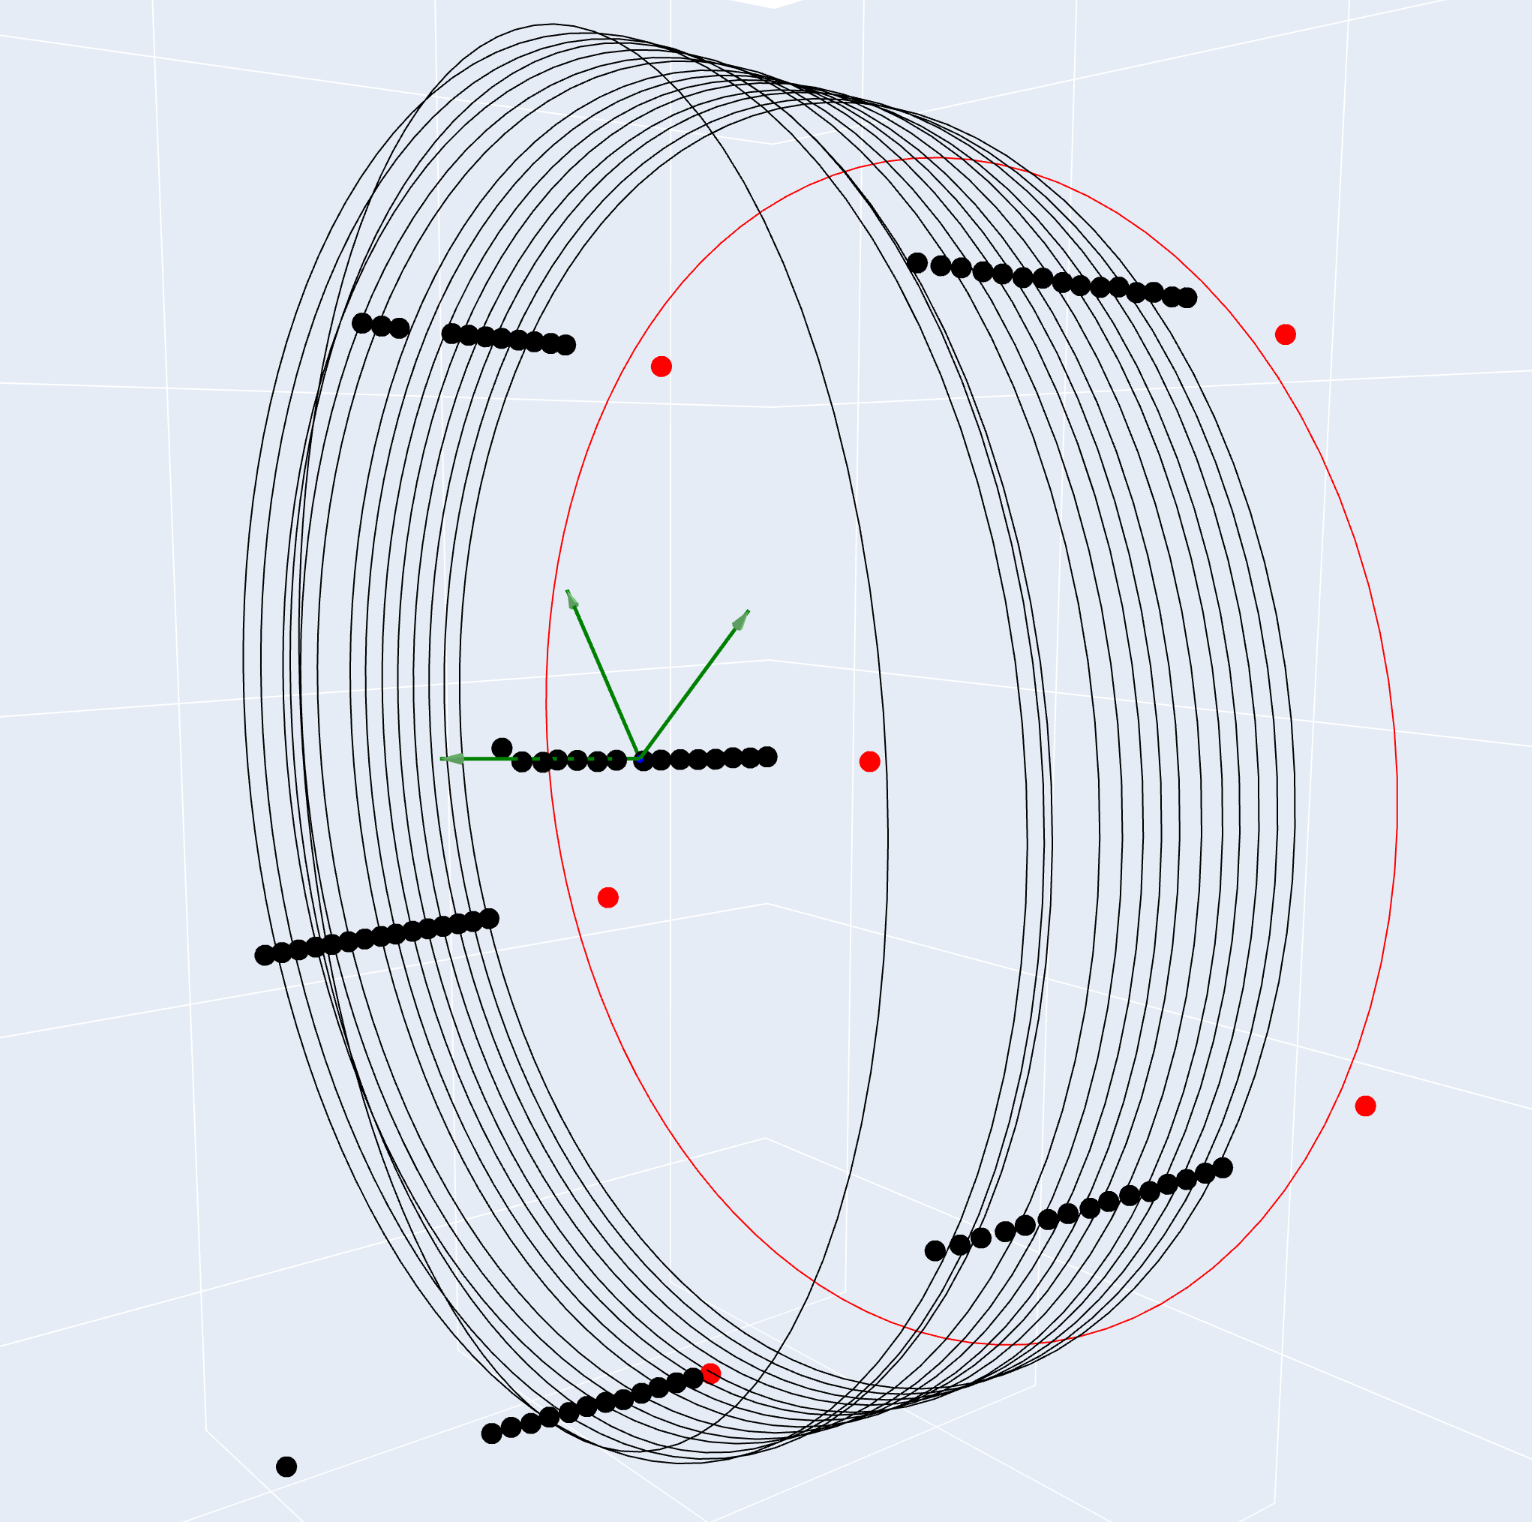
\includegraphics[width=\textwidth]{images/ILUC_naive_grouping.png}
        \caption{Lines 3 to 6 of algorithm \ref{alg:iluc_estimation}. Shown are the ILUC rib edge points grouped into possibly mismatched ILUC rib edges. The mismatched ILUC rib edges result in slanted circles. The midpoints of these circles are used to estimate the ILUC direction (green vector). One set of ILUC rib mid- and edge points are marked in red, since these points were determined to be outliers.}
        \label{fig:iluc_mismatched_edges}
    \end{subfigure}
    \begin{subfigure}[c]{0.45\textwidth}
        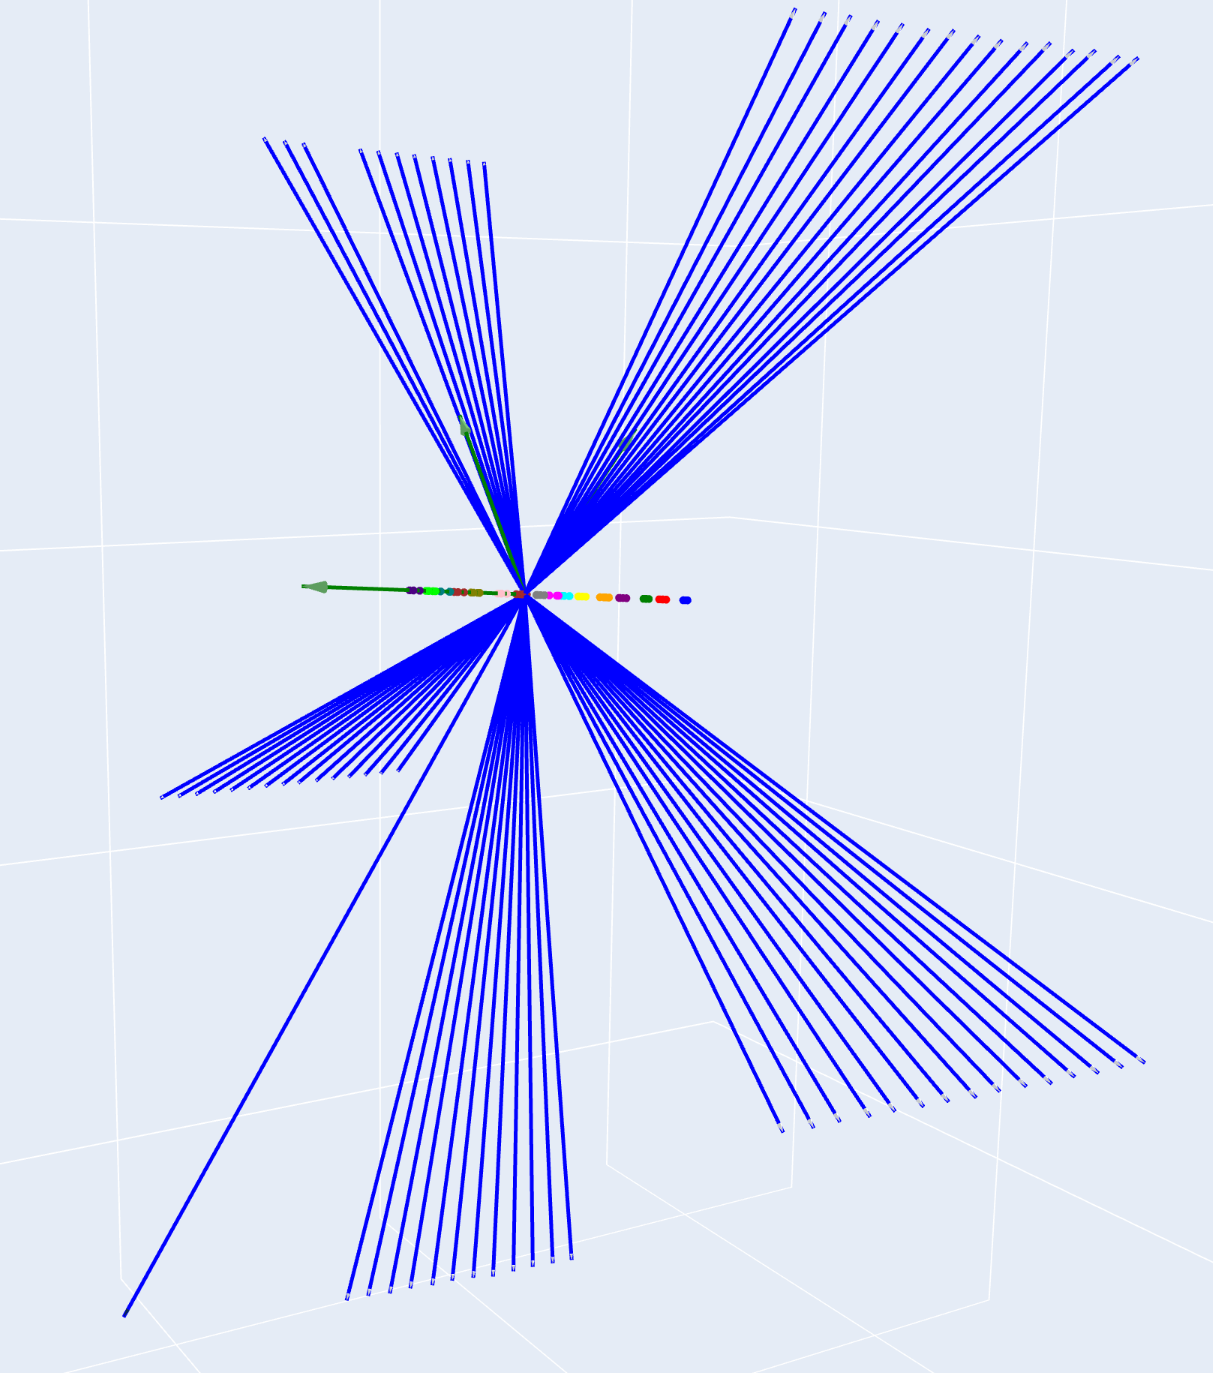
\includegraphics[width=\textwidth]{images/ILUC_center_direction_projections.png}
        \caption{Line 8 from algorithm \ref{alg:iluc_estimation}. Using the approximate direction from figure \ref{fig:iluc_mismatched_edges}, the ILUC rib edge points are correctly matched into edges. The blue lines are vectors eminating from the centroid of the ILUC rib circle midpoints to each of the ILUC rib egde points. These vectors are projected onto the approximate ILUC direction. The ILUC rib edge points are then matched into ILUC edges based on the length of the projections. Each color represents a different ILUC rib edge.}
        \label{fig:iluc_center_direction_projections}
    \end{subfigure}
    \begin{subfigure}[c]{0.45\textwidth}
        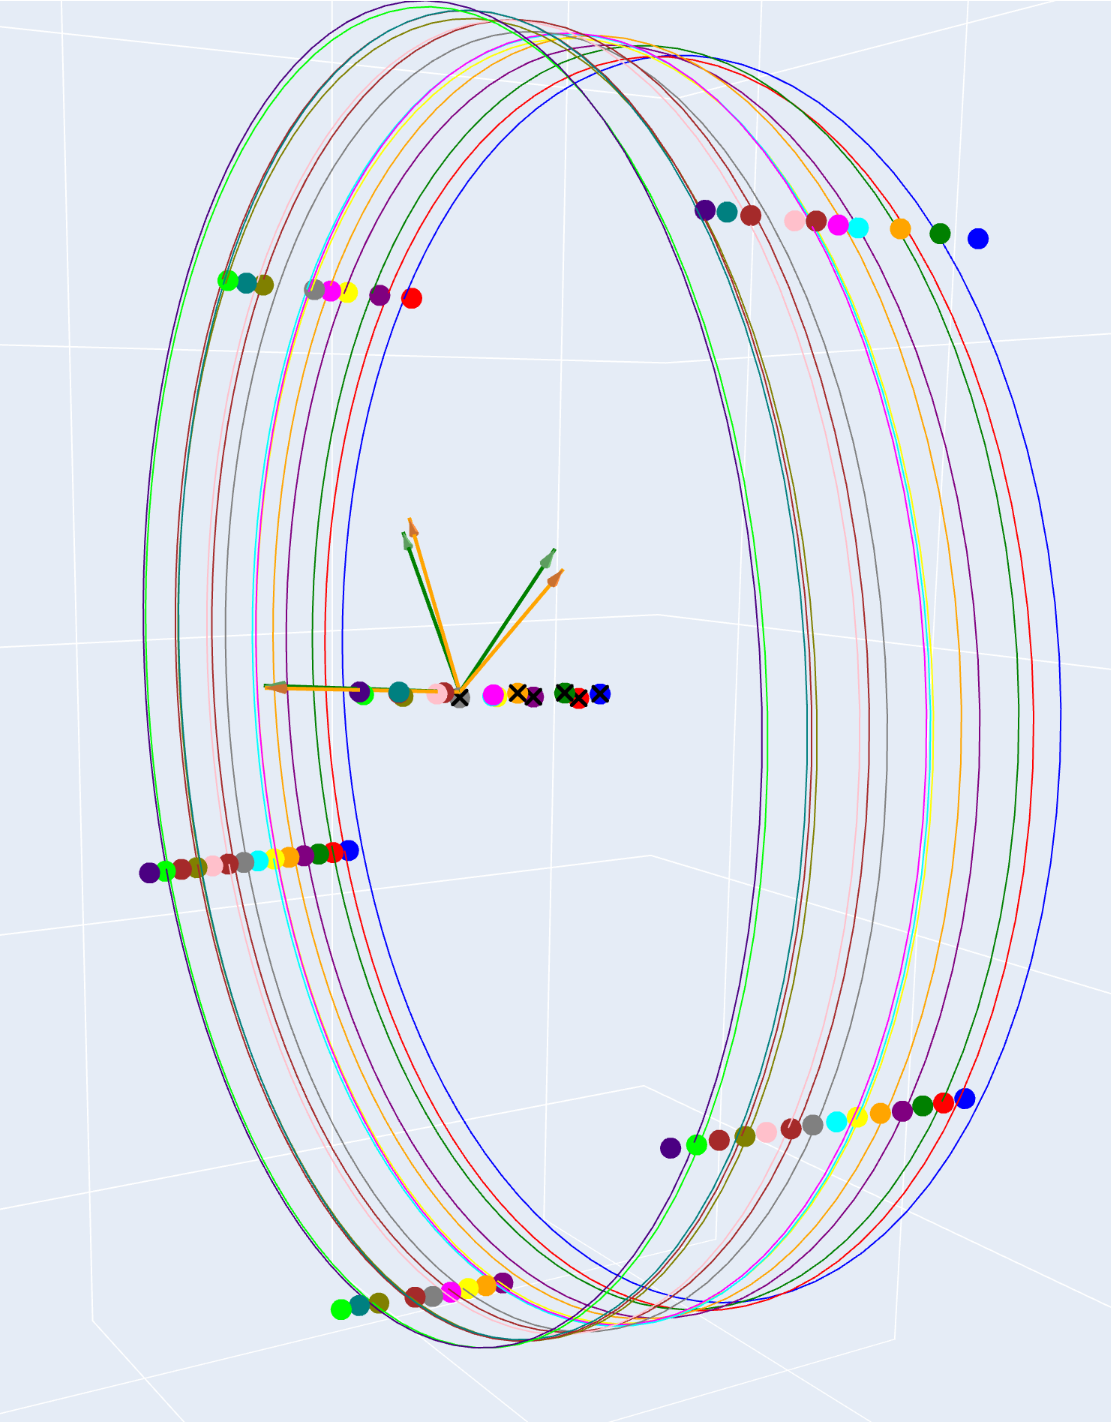
\includegraphics[width=\textwidth]{images/ILUC_matched_edges.png}
        \caption{Line 9 from algorithm \ref{alg:iluc_estimation}. Circles are fit to the correctly matched ILUC rib edges from figure \ref{fig:iluc_center_direction_projections}.}
        \label{fig:iluc_matched_edges}
    \end{subfigure}
    \begin{subfigure}[c]{0.45\textwidth}
        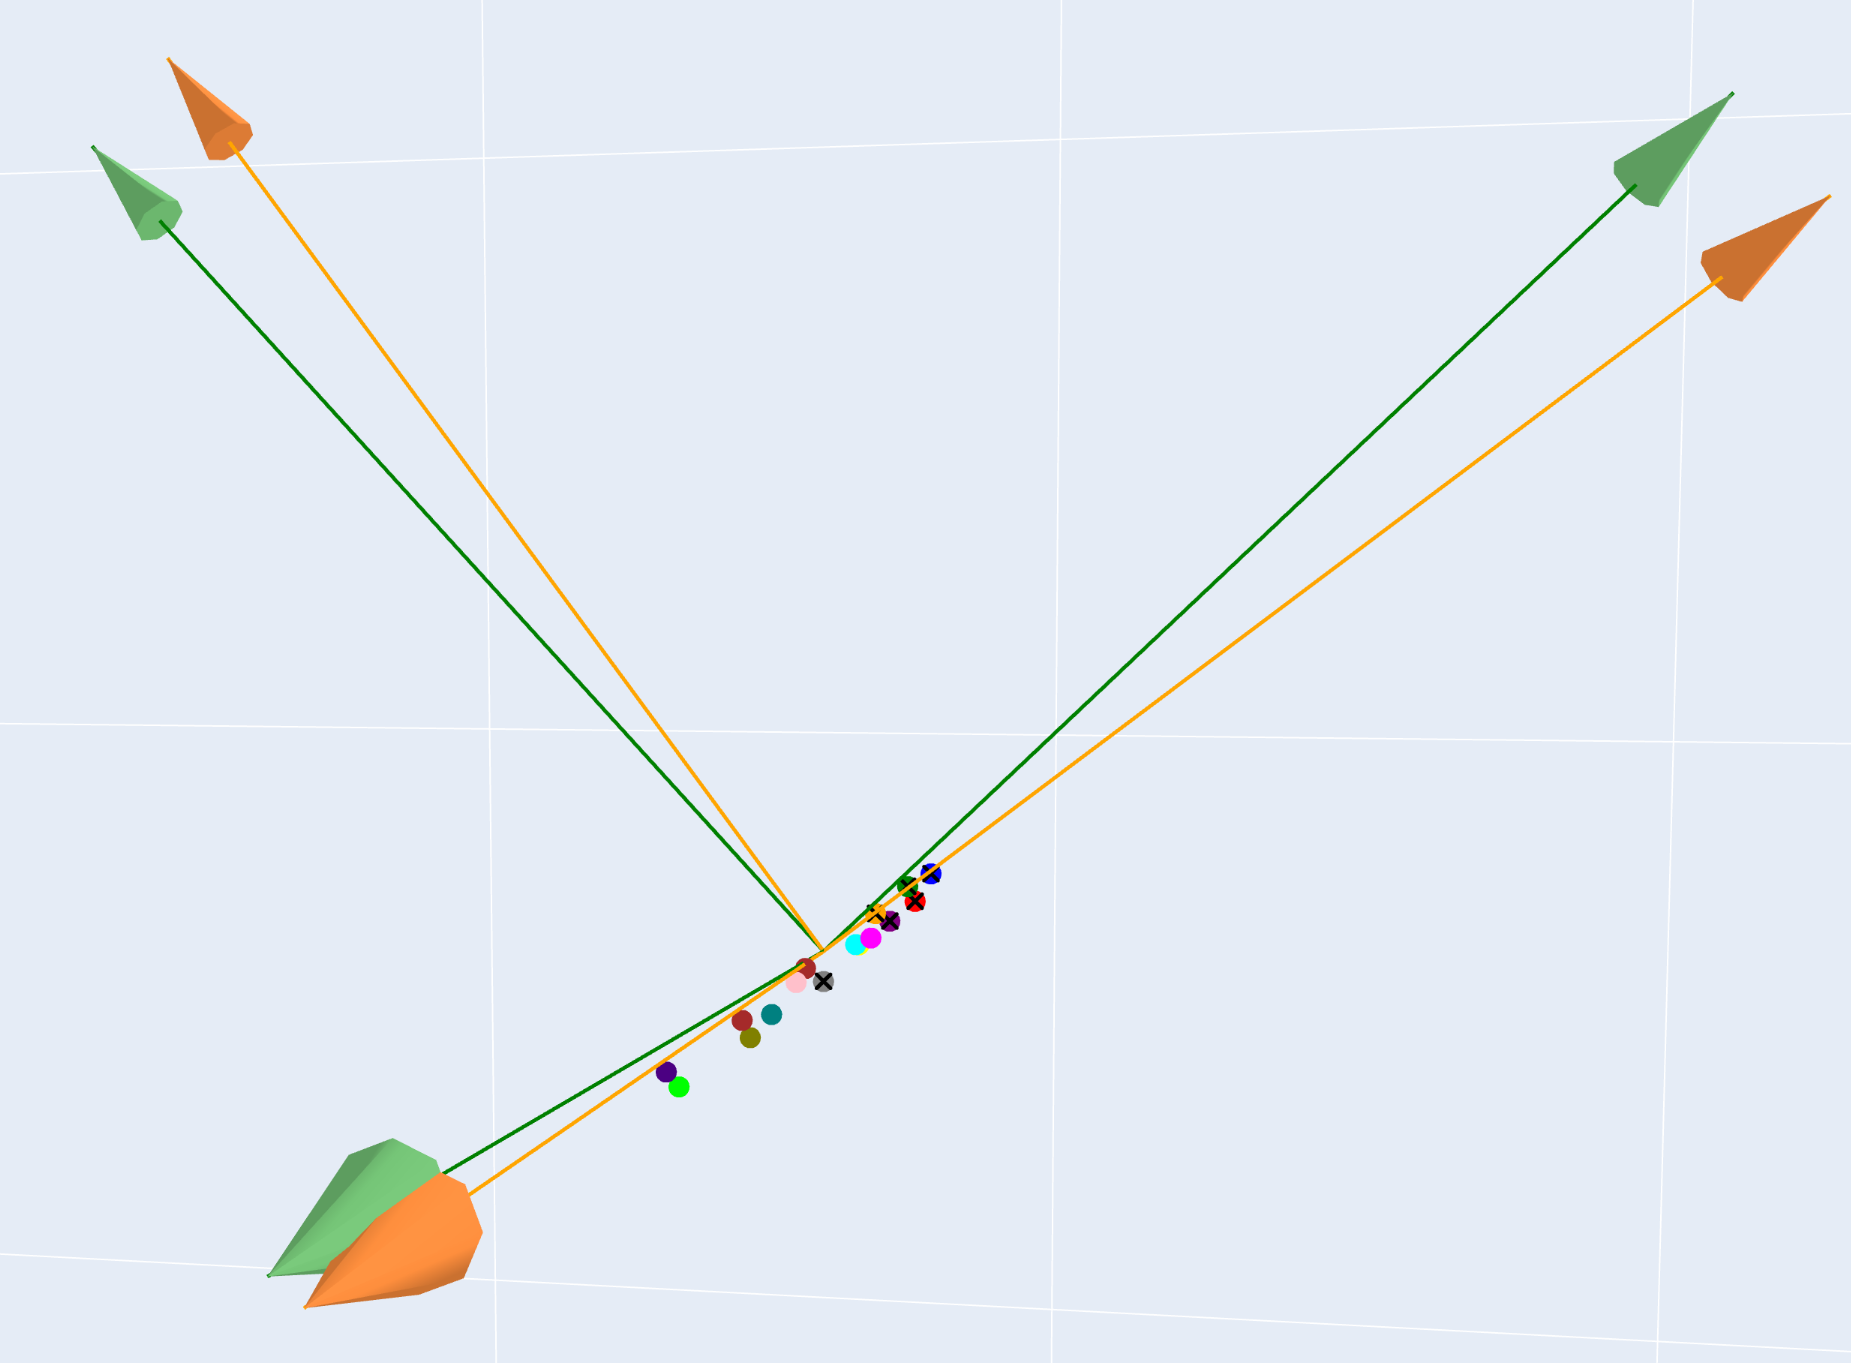
\includegraphics[width=\textwidth]{images/ILUC_corrected_direction.png}
        \caption{Lines 10 and 11 from algorithm \ref{alg:iluc_estimation}. The ILUC rib midpoints from figure \ref{fig:iluc_matched_edges} are filtered for outliers (marked with `$\times$' symbol) and used to obtain a corrected ILUC direction (orange vector). The difference between the corrected and approximate ILUC direction is approximately $0.7^{\circ}$.}
        \label{fig:iluc_corrected_direction}
    \end{subfigure}
    \caption{Visualisation of algorithm \ref{alg:iluc_estimation}.}
    \label{fig:iluc_estimation}
\end{figure}

\subsection{ILUC direction optimisation}
The ILUC direction obtained from algorithm \ref{alg:iluc_estimation} can be further optimised by fitting a cylinder to the ILUC rib edge points. The algorithm is described in algorithm \ref{alg:iluc_optimisation}.
\begin{algorithm}[H]
    \begin{algorithmic}[1]
        \State \textbf{function} \lstinline[language=C]|multiSensorAnalyser_c::fitILUCCylinder|
        \State \textbf{input} ILUC face estimate, ILUC rib edge points without outliers
        \State Use ILUC face estimate to get initial parameters for the cylinder fit $y_c$, $z_c$, $\beta$, $\gamma$, $r$
        \While{a stopping criterion is not met}
        \State Calculate right hand side $\mathbf{\Delta y}$
        \State Calculate Jacobian $\mathbf{J}$
        \State Calculate $\mathbf{C} = \mathbf{J}^T \mathbf{J}$
        \State Calculate condition number $\kappa(\mathbf{C})$
        \State Solve $\mathbf{C} \mathbf{\Delta p} = \mathbf{J}^T \mathbf{\Delta y}$ for $\mathbf{\Delta x}$ $\leftarrow$ Use e.g. Cholesky decomposition, since $C$ is a relatively small (5x5), symmetric matrix
        \State Update parameter vector $\mathbf{p} = \mathbf{p} - \mathbf{\Delta x}$
        \State Calculate loss $l_{i+1}$ and error $e$ of the updated cylinder
        \State Calculate convergence ratio $\rho = \frac{L_i - L_{i+1}}{L_i}$
        \State Update loss $L_i = L_{i+1}$
        \State Update iteration counter $i = i + 1$
        \EndWhile
        \State Convert cylinder parameters to ILUC face; direction, centre and radius
        \State Calculate average error of the ILUC face
        \State \textbf{output: } Optimised ILUC face, average error
    \end{algorithmic}
    \caption{Pseudo code for ILUC face optimisation.}
    \label{alg:iluc_optimisation}
\end{algorithm}
The `stopping criterion' in algorithm \ref{alg:iluc_optimisation} refers to one of the following conditions:
\begin{itemize}
    \item The maximum number of iterations is reached: $i > i_{max} = 100$.
    \item The error becomes smaller than a certain threshold: $e < e_{\text{min}} = 5\times10^{-4} = 0.5 \text{mm}$.
    \item The perdentual change of the loss function is smaller than a certain threshold: $\rho < \rho_{\text{min}} = 10^{-4} = 0.01\%$.
    \item The loss and/or error becomes NaN.
    \item The condition number of the Jacobian matrix is too high: $\kappa > \kappa_{\text{max}} = 10^6$. This indicates that the routine has either converged to a minimum, is stuck in a local minimum or is stuck on a flat region of the loss function.
\end{itemize}
The values of the thresholds are chosen based on the expected accuracy of the ILUC face and the computational resources available. The thresholds are chosen such that the optimisation routine converges within a reasonable amount of time and the ILUC face is accurate enough for the purposes of the LUA software.

\subsection{Cylinder fit model}
The algorithm \ref{alg:iluc_optimisation} is based on a non-linear least squares formulation of fitting a cylinder centered around the $x$-axis. The model equation for a cylinder of this kind is given by
\begin{equation}
    f(\vec{x},\vec{p}) = r^2 - Y^2 - Z^2,
    \label{eq:cylinder_model}
\end{equation}
where $r$ is the radius of the cylinder, $Y$ and $Z$ are the coordinates of the ILUC rib edge points in the $y$ and $z$ direction respectively and $\vec{p} = (y_c, z_c, \beta, \gamma, r)$ are the parameters of the cylinder. The parameters $y_c$ and $z_c$ are the coordinates of the cylinder centre in the $y,z$-plane, $\beta$ and $\gamma$ are the angles of the cylinder with respect to the $y$ and $z$ axes respectively. The model for the cylinder is shown in figure \ref{fig:cylinder_model}.
\begin{figure}[H]
    \centering
    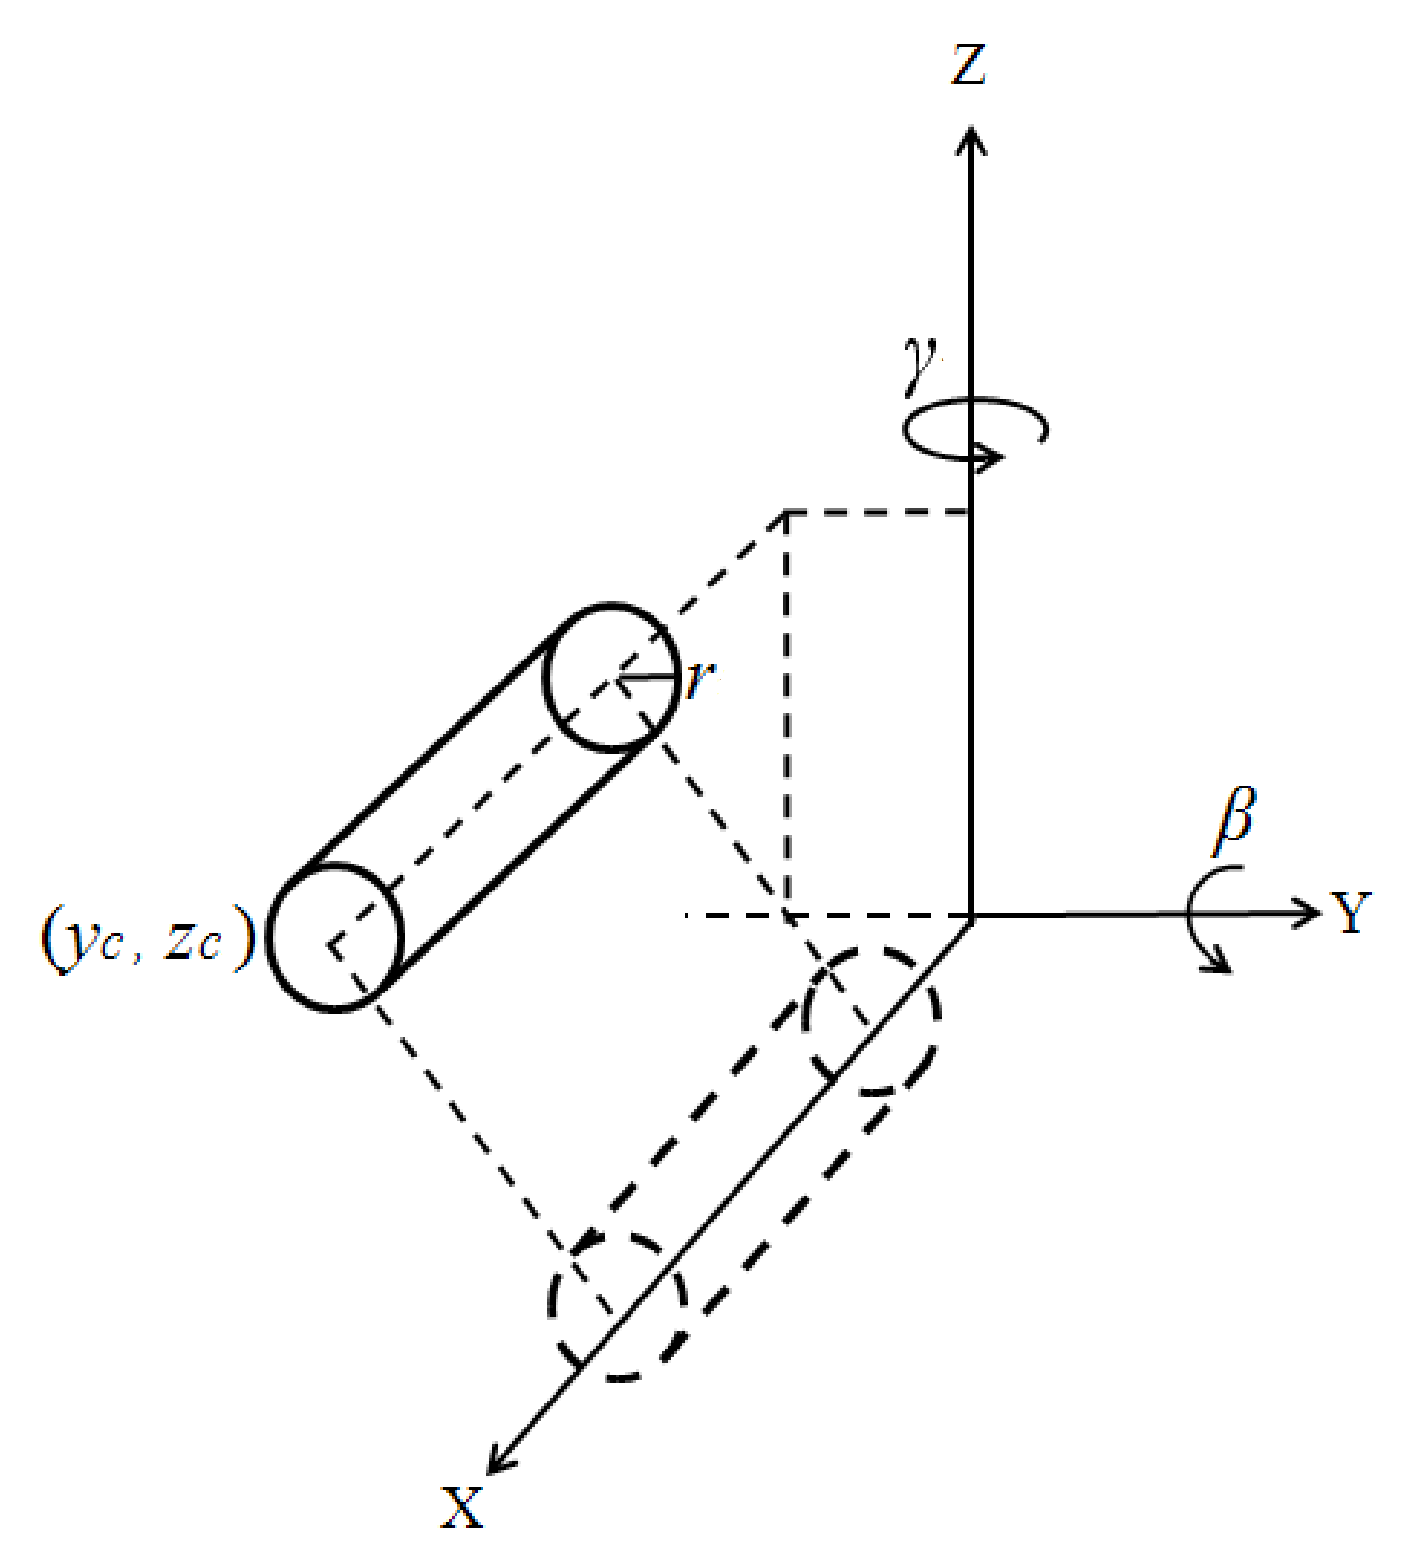
\includegraphics[width=0.6\textwidth]{images/cylinder_model.png}
    \caption{Model of the cylinder used in algorithm \ref{alg:iluc_optimisation}. The cylinder is centered around the $x$-axis and has radius $r$. The coordinates of the cylinder centre $y_c$ and $z_c$ in the $y$ and $z$ direction respectively. The cylinder is rotated by angles $\beta$ and $\gamma$ with respect to the $y$ and $z$ axes respectively \cite[figure 2]{cylinder_fit}.}
    \label{fig:cylinder_model}
\end{figure}
The variables $Y,Z$ in equation \ref{eq:cylinder_model} represent the coordinates of the ILUC rib edge points in the cylinder's frame of reference and are given by
\begin{equation}
    \begin{pmatrix}
        X \\
        Y \\
        Z
    \end{pmatrix} =
    R_y(\beta) R_z(\gamma) \begin{pmatrix}
        x       \\
        y - y_c \\
        z - z_c
    \end{pmatrix},
    \label{eq:cylinder_coordinates}
\end{equation}
where $R_y(\beta)$ and $R_z(\gamma)$ are rotation matrices around the $y$ and $z$ axes and $\vec{x} = (x, y, z)^T$ is the coordinate of an ILUC rib edge point respectively \cite[equation 5]{cylinder_fit}.
The residual function of the model is given by
\begin{equation}
    R(\vec{x},\vec{p}) = -f(\vec{x},\vec{p}) = -(r^2 - Y^2 - Z^2).
    \label{eq:cylinder_residual}
\end{equation}

The loss function is defined as the sum of the squared residuals
\begin{equation}
    L = \sum_{j=1}^{N} R_j^2,
    \label{eq:cylinder_loss}
\end{equation}
where $N$ is the number of ILUC rib edge points. The loss function is minimised by adjusting the parameters $\vec{p}$ of the cylinder. This is done by solving the normal equations
\begin{equation}
    \mathbf{J}^T \mathbf{J} \mathbf{\Delta p} = \mathbf{J}^T \mathbf{\Delta y},
    \label{eq:cylinder_normal_equations}
\end{equation}
where $\mathbf{J} \in \mathbb{R}^{(N\times5)}$ is the Jacobian matrix of the residuals of the ILUC rib edge points with respect to the parameters $\vec{p}$ and $\mathbf{\Delta y}\in\mathbb{R}^N$ is the right hand side of the normal equations. The Jacobian matrix is given by
\begin{equation}
    \mathbf{J}_{jk} = \frac{\partial R(\vec{x}_j, \vec{p})}{\partial p_k},
\end{equation}
where $j$ is the index of the ILUC rib edge point and $k$ is the index of the parameter. Then, the right hand side of the normal equations is given by
\begin{equation}
    \mathbf{\Delta y}_j = R(\vec{x}_j, \vec{p}).
    \label{eq:cylinder_rhs}
\end{equation}

A major assumption of this model is that the cylinder is close to the $x$-axis. This is in fact the case for the ILUC in the coordinate system of the LUA software.

Furthemore, the initial parameters cannot be too far off from the minimizing parameters, because algorithm \ref{alg:iluc_optimisation} is iterative. A bad initial guess can lead to slow (sub-quadratic) convergence, local minima or divergence. However, the initial parameters of the cylinder are obtained from the ILUC face estimate resulting from algorithm \ref{alg:iluc_estimation}. Hence, the initial parameters are already close to the minimizing parameters.

\subsection{ILUC face accuracy}
Table \ref{table:iluc_recognition_accuracy} shows the accuracy of the ILUC face recognition algorithm for various data sets of the ILUC. `stationary' refers to the ILUC being stationary, while `oscillating (XY)' and `oscillating (XZ)' refer to the ILUC oscillating in the $y$-$z$ plane and $x$-$z$ plane respectively. The table shows that the ILUC face recognition algorithm is able to accurately estimate the ILUC face for all data sets.
\begin{table}[H]
    \centering
    \begin{tabular}{|p{1.8cm}||p{1.8cm}|p{1.8cm}|p{1.8cm}|p{1.8cm}|p{2.3cm}|}
    \hline
    \textbf{Data Set} & \textbf{ILUC Face Recognition \%} & \textbf{Average Error (mm)} & \textbf{Optimise Success \%} & \textbf{Optimised Average Error (mm)} & \textbf{Improvement \%} \\
    \hline
    stationary & 100 \% & 0.699 & 38.8\% & 0.215 & 33.5\% \\
    \hline
    oscillating (XY) & 85.8\% & 0.806 & 34.4\% & 0.172 & 23.5\% \\
    \hline
    oscillating (XZ) & 87.7\% & 1.09 & 41.7\% & 0.238 & 28.3\% \\
    \hline
    \end{tabular}
    \caption{ILUC Recognition Accuracy. \textbf{ILUC Face Recognition \%} is the percentage of ILUC faces succesfully recognised. \textbf{Average Error (mm)} is the average error of the estimated ILUC faces. \textbf{Optimise Success \%} is the percentage of ILUC faces successfully optimised. \textbf{Optimised Average Error (mm)} is the average error of the optimised ILUC faces. \textbf{Improvement \%} is percentage of times the optimisation routine resulted in a smaller average error than the estimated case. Note, optimisation can introduce a larger error, if the initial estimate was already very close to the true value.}
    \label{table:iluc_recognition_accuracy}
    \end{table}